\documentclass[a4paper,12pt]{article}
\usepackage{graphicx}
\usepackage{titlesec}
\usepackage[utf8]{inputenc}
\usepackage{xcolor}
\usepackage{fancyhdr}
\usepackage{lipsum}
\usepackage{caption}
\usepackage{amsmath}
\usepackage[a4paper,%
left=0.5in,right=0.5in,top=0.35in,bottom=0.8in,%
footskip=.25in]{geometry}

\renewcommand{\headrulewidth}{0pt}
\fancyhead[C]{}
\fancyhead[C]{
	
\includegraphics[width=4cm]{metu}
}
\pagestyle{plain}

%opening
\title{Middle East Technical University\\Department of Physics\\\textbf{PHYS307 Applied Modern Physics}}
\author{Oğuzhan ÖZCAN\\1852334}
\date{}
\clearpage
\thispagestyle{empty}
\providecommand{\groupmember}[1]{\textbf{Group Members:} }
\providecommand{\expdate}[1]{\textbf{Experiment Date:} }
\providecommand{\repdate}[1]{\textbf{Report Submit Date:} }
\providecommand{\expname}[1]{\textbf{Exp. MP-SB The Spectroscopy of Beta $\beta$ Particles} }



%\topmargin -4.5cm
%\oddsidemargin 0.2cm
%\textwidth 16cm %
%\textheight 21cm%
%\footskip 1.0cm%




\begin{document}
\pagenumbering{gobble}
\maketitle

\thispagestyle{fancy}

%%%%%%%%%%%%%%%%%%%%%%%%%%%%%%%%%%%%%%%%%%%%%%%%%%%%%
\noindent\rule{18.4cm}{0.8pt}
\begin{center}
	\expname{arg1}{}
\end{center}
\groupmember{arg1}{Cem MADEN, İrem KÜL, Deniz AKYÜREK}\\
\expdate{arg1}{November 13, 2015}\\
\repdate{arg1}{November 20, 2015}\\
\noindent\rule{18.4cm}{0.8pt}\\\\
%%%%%%%%%%%%%%%%%%%%%%%%%%%%%%%%%%%%%%%%%%%%%%%%%%%%%
\begin{table}[h!]
	
	\begin{center}
		\begin{tabular}{|c|c|c|c|}
			\hline \textbf{Trial 1} & \textbf{Trial 2}  & \textbf{Trial 3}  & A\textbf{verage Counts} \\ 
			\hline 4 & 5 & 7 & 5.33 \\ 
			\hline 
		\end{tabular}
		\caption{Counts at zero magnetic field \textit{(B=0)} strength for $^{90}$Sr}
	\end{center} 
\end{table}

\begin{table}[h!]
	\begin{center}
\begin{tabular}{|c|c|c|c|c|c||c|}
	\hline \textbf{B [mT]} & \textbf{Trial 1} & \textbf{Trial 2}  & \textbf{Trial 3} & \textbf{Average} & \textbf{Corrected Average} & \textbf{Energy [keV]   } \\ 
	\hline 10 & 11 & 9 & 5 & 8.33 & 3 & 21.48 \\ 
	\hline 20 & 16 & 16 & 13 & 15 & 9.67 & 81.41 \\ 
	\hline 30 & 14 & 19 & 21 & 18 & 12.67 & 169.16 \\ 
	\hline 40 & 27 & 19 & 21 & 22.33 & 17 & 276.83 \\ 
	\hline 50 & 52 & 37 & 45 & 44.67 & 39.34 & 396.20 \\ 
	\hline 60 & 52 & 62 & 55 & 56.33 & 51 & 523.57 \\ 
	\hline 70 & 66 & 69 & 67 & 67.33 & 62 & 656.32 \\ 
	\hline 80 & 64 & 90 & 75 & 76.33 & 71 & 792.82 \\ 
	\hline 90 & 85 & 71 & 83 & 79.66 & 74.33 & 932.02 \\ 
	\hline 100 & 86 & 66 & 78 & 76.66 & 71.33 & 1073.16 \\ 
	\hline 110 & 98 & 59 & 85 & 80.66 & 75.33 & 1215.80 \\ 
	\hline 120 & 59 & 70 & 69 & 66 & 60.67 & 1359.60 \\ 
	\hline 130 & 58 & 58 & 60 & 58.66 & 53.33 & 1504.3 \\ 
	\hline 140 & 35 & 49 & 32 & 38.66 & 33.33 & 1649.73 \\ 
	\hline 150 & 34 & 26 & 27 & 29 & 23.67 & 1795.74 \\ 
	\hline 160 & 32 & 29 & 20 & 27 & 21.67 & 1942.23 \\ 
	\hline 170 & 19 & 14 & 12 & 15 & 9.67 & 2089.12 \\ 
	\hline 180 & 12 & 10 & 9 & 10.33 & 5 & 2236.15 \\ 
	\hline 190 & 6 & 9 & 11 & 8.66 & 3.33 & 2383.86 \\ 
	\hline 199.5 & 6 & 7 & 7 & 6.66 & 1.33 & 2531.61 \\ 
	\hline 
\end{tabular} 
\caption{Counts of $\beta^{-}$-particles for different values of magnetic field strength}
\end{center} 
\end{table}
We need to calculate kinetic energy of each particle in different magnetic fields. The kinetic energy $K$ of a particle is
\begin{equation}
K=\sqrt{(eBrc)^{2}+m_{0}^{2}c^{4}}-m_{0}c^{2}
\end{equation} 
where $e$ is charge of an electron, $r$ is radius of given orbital, $c$ is speed of light, $B$ is magnetic field and $m_{0}$ is rest mass of particle. As an example for a kinetic energy of a $\beta^{-}$-particle, we can take a particle which is in B=100 mT magnetic field. We are going to use following values:\\\\
\textbullet \space $e=1.60217662\times10^{-19}$ C\\
\textbullet \space $m_{0}=9.10938215\times10^{-31}$ kg\\
\textbullet \space $r=0.05$ m\\
\textbullet \space $c=3.0\times10^{8}$ m/s\\
\textbullet \space $B=0.1$ T
\begin{equation}
\begin{split}
K=&\sqrt{(1.60217662\times10^{-19}\times 0.1\times 0.05 \times 3.0\times10^{8})^{2}+(9.10938215\times10^{-31})^2(3.0\times10^{8})^{4}}-\\  
& (9.10938215\times10^{-31})(3.0\times10^{8})^{2}
\end{split}
\end{equation}
\begin{equation}
K=\sqrt{6.45\times10^{-26}}-8.20\times 10^{-14}
\end{equation}
\begin{equation}
K=2.53923\times 10^{-13}-8.20\times 10^{-14}
\end{equation}
\begin{equation}
	K=1.72 \times 10^{-13} Joule
\end{equation}
As we can see, this equation gives result in Joules unit. However, we need to convert it to keV. Therefore we are going to use following equation:
\begin{equation}
	1 J = 6.2415096471204 \times 10^{15} keV
\end{equation}
Finally, we see that at 100 mT magnetic field, a $\beta^{-}$-particle has a kinetic energy of 1073.16 keV.\\\\\\
Experimental end-point energy of $\beta^{-}$-particles = 2531.61 keV\\\\
Accepted end-point energy of $\beta^{-}$-particles = 2270 keV\\\\
Percentage error in end-point energy of $\beta^{-}$-particles = 3.59\% \\
\begin{equation}
Percentage Error=\frac{|Experimental Value-Theoretical Value|}{Theoretical Value}\times 100\%
\end{equation}\\\\
\textbf{1. Explain the high counting readings when the magnetic field strength is equal to zero.}\\\\
Background counting is caused by different types of radiation and their penetrating ability. These may be natural sources such as cosmic rays and
radioactive elements found in the surrounding air and building materials, or
artificial sources such as unshielded radioactive chemicals stocked nearby or the
luminous paint of a wristwatch [1]. For instance, in our lab we have Cs-137 and it can cause some radiation. The background radiation count rate should always
be measured as part of any radiation experiment. It should then be subtracted from
the count rate data taken for the experimental source like as we did while calculating corrected average. In fact, there is a way to reduce background radiation. C-14  is a good beta emitter but in our experiment it does not work because its beta
particles have low energy and are deflected out of the magnetic field before
they can reach the Geiger tube [2].
\newpage
Another possible background counting cause may be Bremsstrahlung \textit{(also known as braking radiation or deceleration radiation)}. Bremsstrahlung is a electromagnetic radiation which is produced by the deceleration of charged particles when these particles deflected by another particle [3]. Since I am not familiar with this topic, I will not move deeper.\\\\
\textbf{2. Comment on the graph that you have plotted.}\\\\
\begin{figure}[h!]
\centering
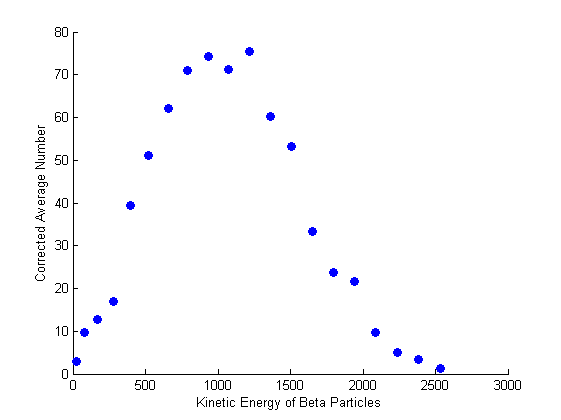
\includegraphics[width=0.7\linewidth, height=0.35\textheight]{g1}
\caption{Corrected average number versus kinetic energy of $\beta^{-}$-particles emitted from Sr-90 in keV}
\label{fig:g1}
\end{figure}
This graph demonstrate the spectrum of electrons emitted in the $\beta^{-}$ decay of Sr-90. The last data point shows us the endpoint of Sr-90. Since we have some experimental error our graph does not look like theoretical one. These graphs are mostly plotting in MeV unit but we plotted in keV. In this experiment we used only Sr-90. However, this experiment completed with other elements such as Cs-137, Co-60 and Am-241. Note that each one will give different graphs. For instance, we have only one peak but Cs-137 and Co-60 have more than two peaks (see Figure 2).
\begin{figure}[h!]
\centering
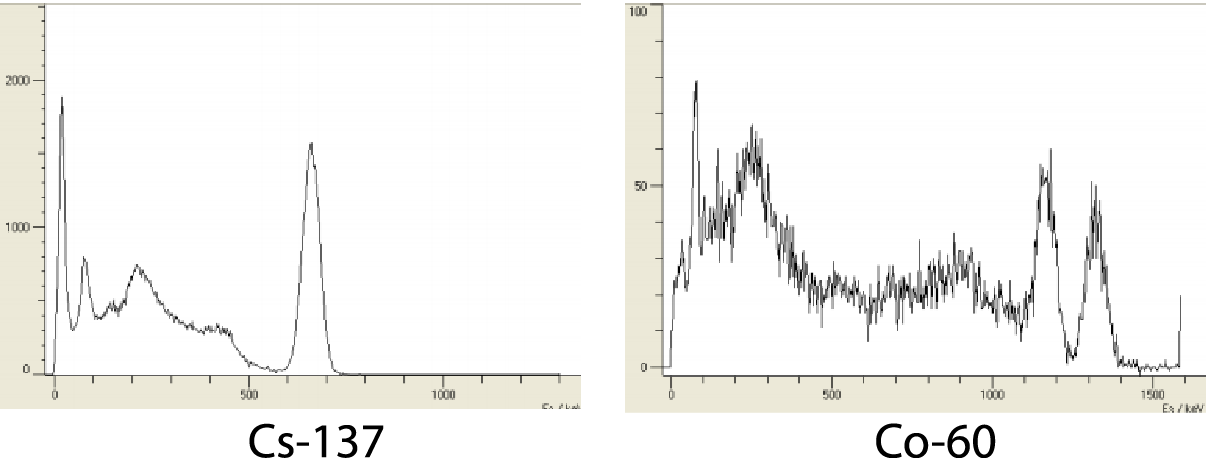
\includegraphics[width=0.7\linewidth, height=0.2\textheight]{21321}
\caption{Spectrum for Cs-137 and Co-60 with Background Subtracted}
\label{fig:21321}
\end{figure}

\newpage
\textbf{Discussion and Conclusion}\\\\
In this experiment, we studied the $\beta^{-}$-particle decay which is very important topic in nuclear physics. This experiment shows that kinetic energy of $\beta$ particles can effected by magnetic field. Besides, each radioactive isotopes have different kinetic energy values and different energy spectrum also. Another important fact that I learned in the experiment is that a radioactive isotope can transform another radioactive isotope at different kinetic energies. For instance, Sr-90 is a radioactive isotope of Strontium and Sr-90 becomes Yr-90 in 540 keV and then becomes Zr-90 in 2270 keV [4]. After this experiment I became more familiar with some topics such as neutrino, anti-neutrino, Kurie plot and Fermi Function. According to our results, end-point energy of $\beta^{-}$-particles is 2531.61 keV. However, while I was searching this value stated as 546 keV [5]. I am still confused about this value. When examine our graph we can see that we have a peak at 1215 keV kinetic energy and I do not know what does it stands for? If we had more than one source, we would see different behaviours of radioactive isotopes and different energy spectrums. Overall, I think that this experiment was succesful and objective of experiment is reached.\\\\\\

\textbf{References}\\\\
$[1]$ Irodov, I. (1983). \textit{Problems in Atomic and Nuclear Physics} (pp. 82-83). Moscow: Mir.\\\\
$[2]$ Bodansky, D. (2004). \textit{Nuclear Energy - Principles, Practices, and Prospects} (2nd Edition) (2nd ed., p. 634). S.l.: Springer - Verlag.\\\\
$[3]$ Haug, E., \& Nakel, W. (2004). \textit{The Elementary Process of Bremsstrahlung} (pp. 29-30). River Edge, NJ: World Scientific.\\\\
$[4]$ Wong, S. (1998). \textit{Introductory Nuclear Physics} (2nd ed., p. 208). New York: J. Wiley.\\\\
$[5]$ C. Çeliktaş, \textit{Beta Spectrometers with Surface Barrier Detector
and Plastic Scintillator: Applications to
$^{90}$Sr,$^{204}$Tl, $^{210}$Pb and $^{14}$C.}, Turk J Phy
\textbf{25} (2001) , 97 – 107.





































































































































\end{document}
